\subsection{DynamicSTGNN (RQ2-ii)}
\label{sec:dynamic-team-graph-model}

Part (ii) of RQ2 asks whether the dynamic team graphs of
Subsection~\ref{sec:team-graphs} add predictive signal beyond the team-phase
features. DynamicSTGNN receives
\(X \in \mathbb{R}^{B \times T \times N \times F}\) and
\(A \in \mathbb{R}^{B \times T \times E \times N \times N}\), with \(T{=}8\)
phases, \(N_{\max}{=}128\) teams, \(F{=}66\) node features, and \(E{=}3\)
relation channels; Figure~\ref{fig:dynstgnn-arch} shows the architecture.
\(N_{\max}\) is a padding bound covering the largest team count across modes
(up to 100 in solo); padded nodes carry no edges and are masked throughout.
An input layer embeds each node into a 64-dimensional state \(H\), and two
identical spatio-temporal blocks follow. Each block applies a gated causal
temporal convolution, the heterogeneous graph convolution
\[
H' = \mathrm{ReLU}\Big(\sum_{r\in R} \alpha_r\, \bar{A}_k^r H W_r + H W_0\Big),
\qquad \alpha = \mathrm{softmax}(a),
\]
where \(\bar{A}_k^r\) is the row-normalized adjacency of relation \(r\),
\(W_r\) and \(W_0\) are learned projections, and \(a\) are learned channel
logits, and then a second gated causal temporal convolution with layer
normalization and a residual connection. The channel weights \(\alpha\) are
global scalars rather than phase- or team-conditioned attention; the graph
module is therefore designed to test whether the relation channels contain
additional signal, not to model context-dependent relation importance.

Although the tensor has \(T{=}8\) slots, the model emits one hazard logit per
cut phase \(k=1,\dots,7\). Temporal convolutions are left-causal, layer
normalization is applied over the feature dimension of each team-phase state
(never across time), and padded phases and eliminated teams are masked in
message passing and in the loss. A small head maps each team-phase state to
the next-phase hazard logit of Subsection~\ref{sec:prediction-task}. The full
model has about 0.34M parameters.

\begin{figure*}[t]
\centering
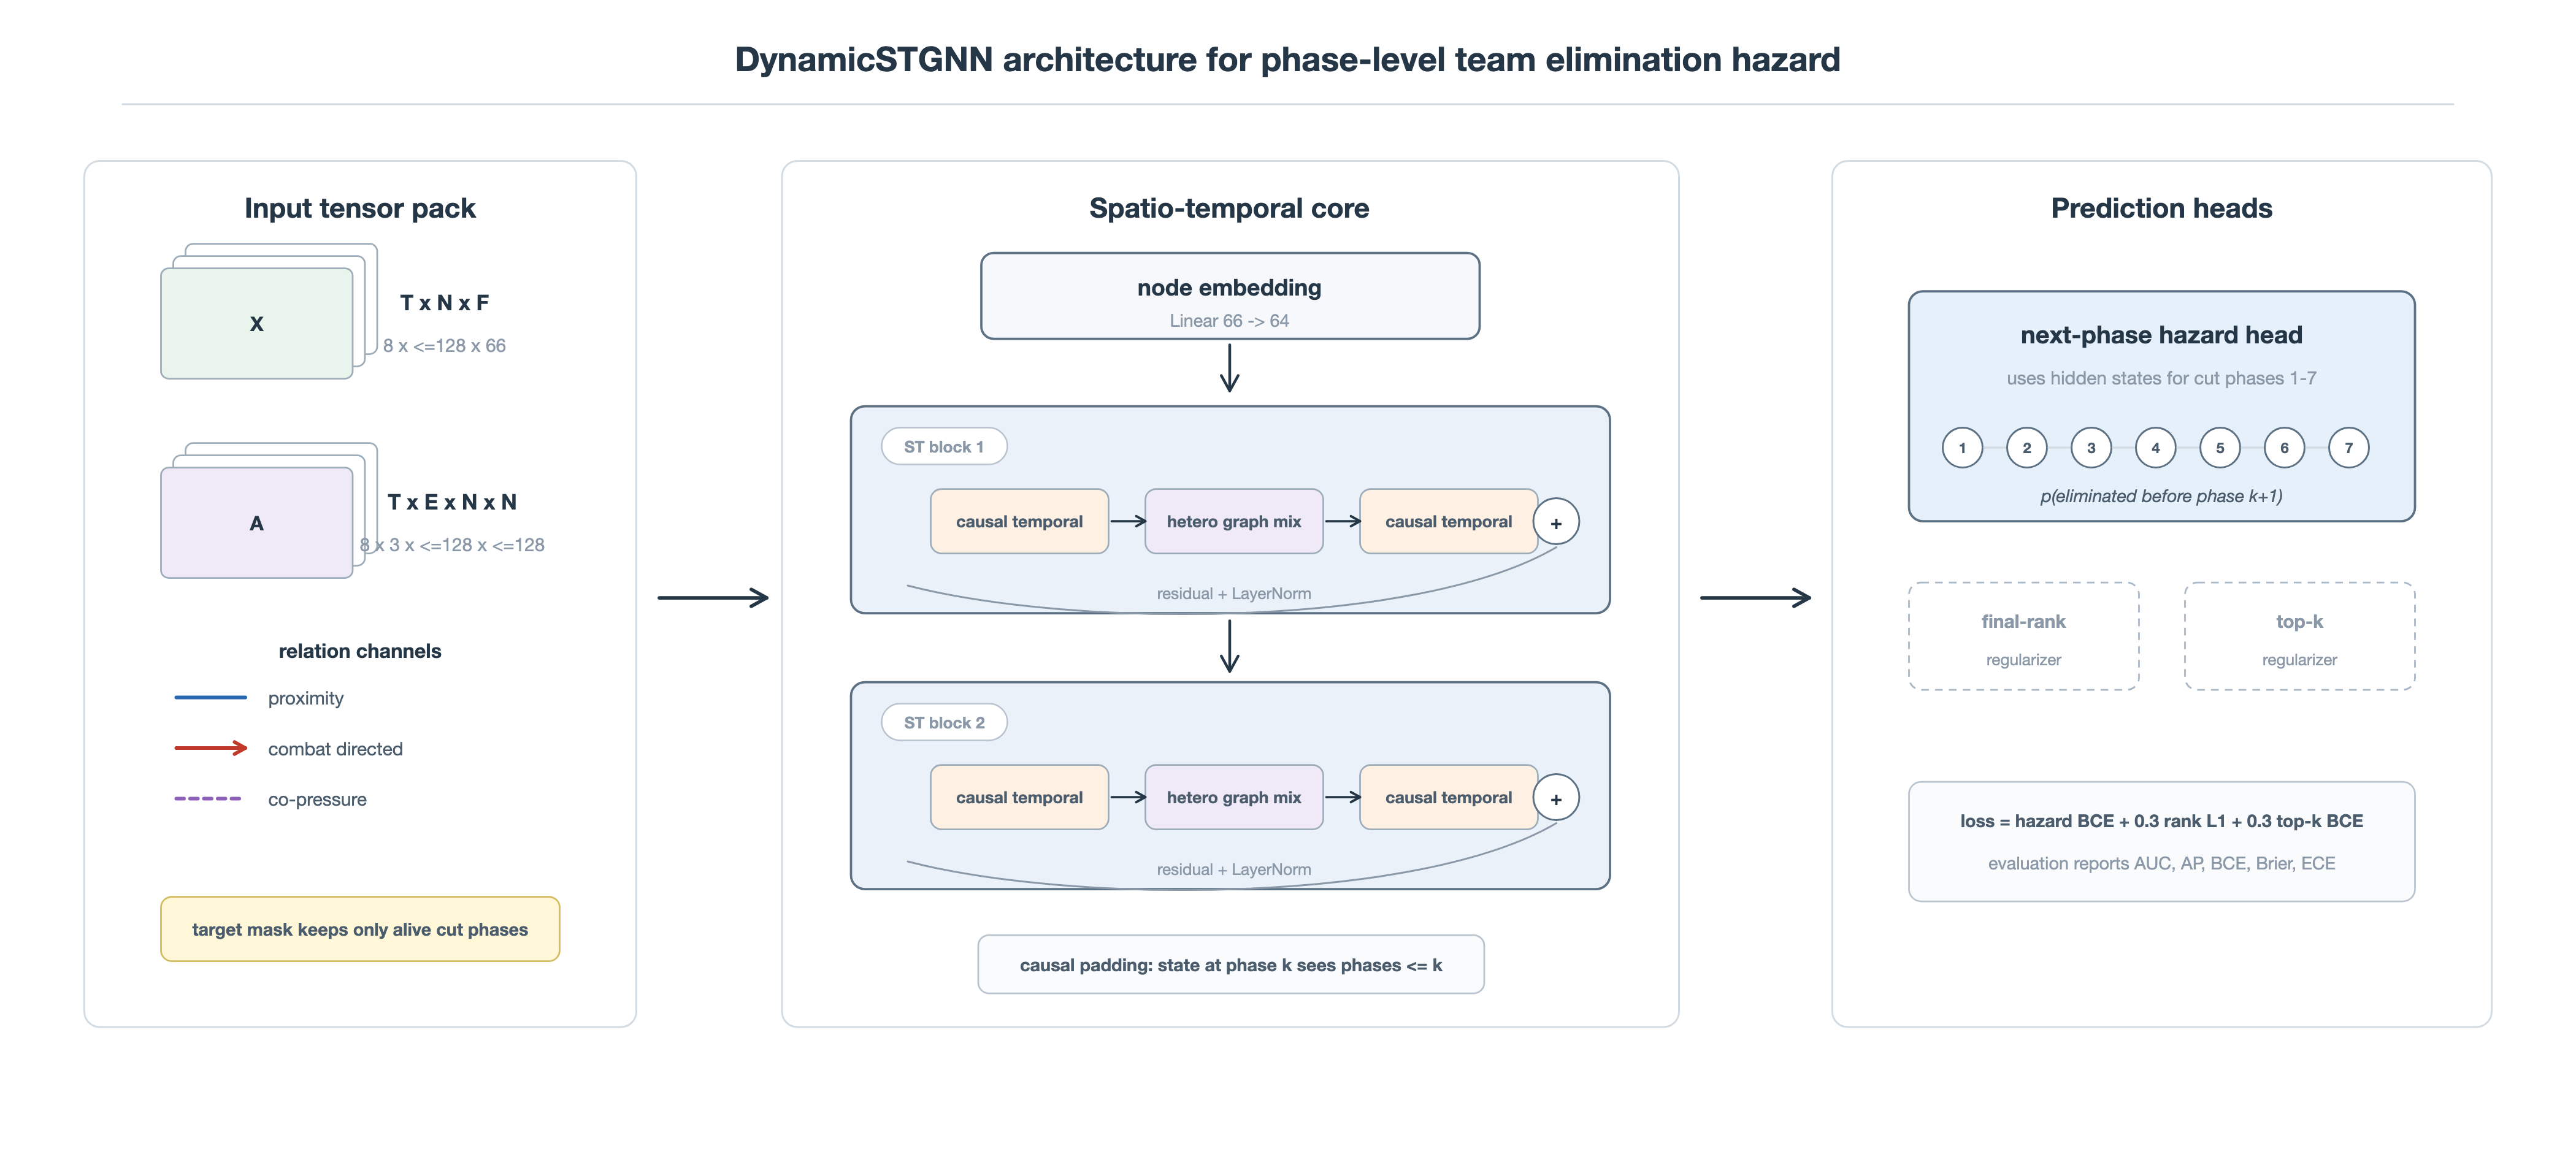
\includegraphics[width=0.86\textwidth]{figures/dynstgnn_architecture.png}
\caption{DynamicSTGNN. (a) The input is one heterogeneous team graph per
phase, with proximity, combat, and co-pressure relation channels. (b) The
network embeds node features and stacks two gated spatio-temporal blocks
before the hazard head. (c) Each ST block applies a gated causal temporal convolution, a heterogeneous graph
convolution that aggregates per relation channel and mixes channels with
learned softmax weights plus a skip connection, a second gated temporal
convolution, and layer normalization with a residual connection. Causal
padding keeps phase \(k\) from seeing later phases.}
\label{fig:dynstgnn-arch}
\end{figure*}

We compare four edge conditions: no edges, proximity only, proximity plus
combat, and the full graph. We also compare against a histogram gradient
boosting baseline on a tabular view of the same team-phase rows. The two
references play distinct roles: the boosting baseline tests whether the graph
model beats a strong tabular learner on the same representation, while the
no-edge DynamicSTGNN controls for architecture, temporal convolution, and
parameter count with relational adjacency removed. Both references already receive hand-crafted neighbor summaries
(nearby enemy density, nearest-enemy distance) among the node features, so
improving on them attributes the gain to relational structure beyond what
such summaries capture. Only gains over both references support the claim
that dynamic team relations add predictive signal. Two controls guard this
conclusion further: shuffling team identities within the observed graphs at
inference time should erase the gain if it truly comes from who relates to
whom, and the gain should persist when training is repeated under different
random seeds.
